\chapter{Theoretische Grundlagen}
%1. Theoretische Grundlagen → als Grundlage für implementierung.
% Was muss der leser wissen, um die realisierung zu verstehen? 
%1. Konkreter, technoloischer: Worum geht es bei plattformunabhängiglkeit, wie ist zu erreichen? → veschiedene grundsätzliche Konzepte
%2. übersicht / Eigenschaften & Einordnung der vorgestellten L\"osungen
%3. Verwendete Technologien → wie macht das phonegap?
%1. Knockout, jquerymobile, etc.

\section{Apps für mobile Geräte}

\subsection{Mobile (native) Apps} \label{native}
Unter mobilen \glspl{app} versteht man im Allgemeinen Anwendungssoftware für Tablet-Computer oder Smartphones. 
Im Laufe der letzten Jahre haben sich auf dem Markt für Mobilgeräte durch viele konkurierende Gerätehersteller eine Vielzahl von Smartphone- und Tablet-Betriebssystemen herausgebildet.
Im Entwicklungsbereich wird in dem Zusammenhang auch von \emph{Plattformen} gesprochen.

Zu den Plattformen mit dem höchsten Marktanteil zählen \glspl{google} Betriebssystem \gls{android}, \gls{ios} von \gls{apple}, \gls{win-phone} und \gls{blackberry-os} des gleichnamigen Smartphone-Herstellers \gls{blackberry-inc} \cite{platforms-marketshare}.
% Nativ-Entwicklung für die jeweiligen Plattformen: Android / iOS
Die \gls{app}-Entwicklung für diese mobilen Betriebssysteme erfolgt mehr oder weniger ähnlich und soll im Folgenden, um auf die beiden größten Vertreter einzugehen, anhand von \gls{android} beziehungsweise \gls{ios} näher beschrieben werden.

%	-> \gls{sdk}s verwalten
Grundsätzlich müssen auf der \gls{ide} die entsprechenden \glspl{sdk} der Plattform, für die entwickelt wird, installiert sein. 
Diese enthalten Softwarekomponenten, die zur Entwicklung der \gls{app} notwendig sind, beispielsweise Klassen, die es einem erlauben, auf native Funktionalitäten des Betriebssystems wie zum Beispiel das Adressbuch, den Benachrichtigungsmechanismus oder auch auf Hardwarekomponenten wie die Kamera, den Bewegungssensor oder das \gls{gps}-Modul zuzugreifen sowie die entsprechenden plattformspezifischen Oberflächenkomponenten des jeweiligen \gls{gui}-Toolkits zu nutzen.

%	-> Code schreiben für die jeweilige Plattform
% Allgemein / Android
Als Programmiersprache für die \gls{android}-\gls{app}-Entwicklung wird \gls{java} verwendet. Das heißt, als Voraussetzung für die Entwicklung von \gls{android}-\glspl{app} ist lediglich eine geeignete \gls{ide} wie \gls{eclipse}, \gls{netbeans} oder \gls{intellij} sowie eine Installation des \gls{java}- und des \gls{android}-\gls{sdk} nötig. 
\todo{wie sieht es mit dem deployment, also der auslieferung in appstores etc aus?}
Seit 2013 bietet Google darüberhinaus die auf \gls{intellij} basierende und eigens für die \gls{android}-Entwicklung angepasste \gls{ide} \gls{android-studio} an \cite{android-studio}, die bereits alle notwendigen Toolkits enthält. 
Nachdem der Code geschrieben ist, kann er kompiliert und zu einem lauffähigen Programm gebaut werden (\seename\ \autoref{fig:hybrid-apps-schaubild}). Anschließend kann die \gls{app} in dem für die Zielplattform vorgesehenen Dateiformat ausgeliefert und auf dem Zielgerät installiert werden.

% iOS: 
Auch der Software- und Computer-Hersteller Apple bietet mit \gls{xcode} eine firmeneigene \gls{ide} zur \gls{app}-Entwicklung für sein mobiles Betriebssystem \gls{ios} an. Anders als Google geht der iPhone-Hersteller hier allerdings etwas restriktiver vor. So läuft die \gls{ide} \gls{xcode}, die man für die native \gls{ios}-Entwicklung benötigt, nur unter dem hauseigenen Betriebssystem \gls{osx} und das wiederum nur auf den firmeneigenen Mac-Rechnern. So sichert sich Apple auch durch jeden Entwickler einen neuen Kunden. \todo{darf man so was hier anmerken, oder lieber weg?}
Ansonsten verläuft der Entwicklungsprozess bei der \gls{ios}-Entwicklung im Prinzip ähnlich zur \gls{android}-Entwicklung (\seename\ \autoref{fig:hybrid-apps-schaubild}).
Als Programmiersprache wird \gls{obj-c} verwendet, einer um objektorientierte Elemente erweiterte Variante der Programmiersprache \gls{c}.

Möchte ein Auftraggeber einer Software also statt seinen Kunden nur eine \gls{app} für ein Betriebssystem anzubieten, einen größeren Nutzerkreis erschließen, muss die zu entwicklende \gls{app} für jede Zielplattform neu programmiert, getestet und gebaut werden, da jede mobile Plattform ihre eigenen Toolkits, Bibliotheken und Programmiersprachen verwendet, was die native \gls{app}-Entwicklung für potenzielle Auftraggeber zu einem sehr kostenaufwändigen Projekt werden lassen kann.
Andererseits bietet die native \gls{app}-Entwicklung vollständige Unterstützung der betriebssystemeigenen Funktionalitäten wie den Zugriff auf Kamera, Adressbuch, Bewegungssensoren etc. der jeweiligen Plattform, sodass ein Softwareprojekt mit solchen besonders hardware- oder betriebssystemnahnen Anforderungen die Entwicklung einer nativen (plattformspezifischen) \gls{app} notwendig erscheinen lassen kann.\footnote{Mehr dazu in \autoref{hybrid}}

\subsection{Web-Anwendungen}\label{web-app}

% Zuerst gab es Websites, dann dynamische websites
Eine \gls{web-app} ist eine Andwendungssoftware, die auf einem Web-Server läuft und auf die der Nutzer mittels eines Browsers zugreifen kann; also eine dynamische Website, wie man sie auch schon vor dem Aufkommen von Smartphones und modernen Tablets kannte. 

Die Grundlage für die Enwicklung von Internetseiten bildet der langjährige Standard \gls{html}, mit dem deren Aussehen, Inhalt und Struktur textuell beschrieben werden kann. 
In Kombination mit \gls{css} für die modulare Gestaltung einer Website sowie \gls{js}, einer Skriptsprache zur \gls{dom}-Manipulation, bietet die HTML-Spezifikation in ihrer neusten Version \textit{(\gls{html5})} im Grunde alles, was für die Entwicklung einer modernen Benutzerschnittstelle am Computer notwendig ist. 
Die Fachlogik liegt, neben den Oberflächen-Komponenten in Form von \mbox{\gls{html}-,} \gls{css}- und Javascript-Dokumenten, auf einem Webserver und verarbeitet und reagiert auf Anfragen des Clients\footnote{hier also des Browsers}.
Als Server-Technologie ist ein breites Spektrum an Programmiersprachen und Umgebungen einsetzbar\footnote{einige sind beispielsweise \gls*{php}, \gls*{java}, \gls*{asp} u.\,v.\,a.\,m.}.

Somit bietet die Entwicklung einer \gls{web-app} (abgesehen von einigen browser-spezifischen Eigenheiten) bereits eine gewisse Plattformunabhängigkeit, da jedes moderne (mobile) Betriebssystem über einen Webbrowser verfügt. 
Zwar müssen Entwickler in bestimmten Details bei der Erstellung des Codes auf die teilweise unterschiedliche Unterstützung (bspw. von \gls{html}-Elementen) \todo{genauer?} durch die verschiedenen Browser achten, aber darüberhinaus wird der Entwicklungsaufwand für eine \gls{web-app} nicht von der Anzahl der Zielplattformen bestimmt, da von Client-Seite aus verschiedene Browser durch die Verbreitung und Beachtung von Web-Standards weitgehend einheitliche \gls{html}-Dokumente lesen und interpretieren können und das Backend nicht auf Clients mit unterschiedlichen Plattformen, sondern auf Webservern liegt, deren Plattform bei der Entwicklung entweder schon bekannt oder nicht relevant ist\footnote{beispielsweise weil auch die Fachlogik plattformunabhängig mit \gls*{php} oder \gls*{java} realisiert wurde}.

% Dann für sämtliche INet-Dienste auch noch eine \gls{app}
Obwohl es, durch damals eher im Business-Bereich verortete Internet-Handys und Palmtops, auch vor den heute üblichen mobilen Touch-Geräten bereits mobile Internetseiten gab, die speziell für die Darstellung auf kleinen Displays ausgerichtet waren, boten mit der massenhaften Verbreitung von mobilen, internetfähigen Geräten und deren (im Folgenden erläuterten) stark anwendungsorientierten Bedien-Konzepten viele herkömmliche Internet-Dienste nun auch zusätzlich eine native \gls{app} für verschiedene mobile Plattformen an.
So sind beispielsweise auch E-Mail-Dienste wie \gls{gmx}, \gls{web-de} oder \gls{gmail} seit der Verbreitung von Smartphones und Tablets auch in Form einer eigenen \gls{app} für \gls{android} und \gls{ios} vertreten, sodass der Nutzer, statt, wie von der Desktop-Computer-Nutzung gewohnt, einen anbieterunabhängigen Mail-Client zu konfigurieren, über den er seine E-Mails abruft, unter Umständen gleich die jeweilige \gls{app} des E-Mail-Anbieters startet \cite{gmx, web.de, gmail}.
Das heißt, der Nutzer folgt einem geänderten Bedienungsmuster seines Mobilgeräts gegenüber der herkömmlichen Computer-Nutzung: um zu einem bestimmten Ergebnis zu gelangen (bspw. \emph{Nachrichten lesen}) also die Frage zu beantworten, \emph{wie} er dahin gelangt (Einen Browser öffnen und zur gewünschten Seite navigieren: www.tagesschau.de), ist es für Anwender heutiger Mobilsysteme naheliegend, gleich die passende \gls{app} zu starten\footnote{hier bspw. die Tagesschau-\gls{app}}.

% Gründe für App statt Web-Anwendung
Dafür gibt es verschiedene mögliche Gründe. Zum Einen muss im Gegensatz zu einer Website bei der mobilen \gls{app} nicht die komplette Oberfläche\footnote{\gls{html}-, \gls{css}- und JavaScript-Dokumente sowie Grafiken} übertragen werden, sondern lediglich die Nutzdaten,\footnote{also beispielsweise, um beim obigen Beispiel zu bleiben, die Nachrichten in Textform.} was dem Nutzer ein höheres Maß an Performanz einbringt.
Zum Anderen können trotz Vollbildmodus in bestimmten Fällen \gls{gui}-Elemente des Webbrowsers bei der Benutzung einer Web-Anwendung störend sein, so ist beispielsweise die Adresszeile am Rand nicht unbedingt erwünscht, wenn der Nutzer statt im Internet zu surfen dort eigentlich eine bestimmte Anwendung nutzen möchte. 
Ein anderes Beispiel für ein eventuell unerwünschtes Verhalten der Benutzerschnittstelle ist das der \emph{Menü}-Taste bei \gls{android}-Geräten, die im Falle der Nutzung einer Web-Anwendung über den Browser nicht den Kontext der eigentlich benutzten Anwendung \footnote{hier also der Website} anzeigt, sondern lediglich den des Browsers.

In bestimmten Fällen kann eine nützliche Funktion einer \gls{app} die Offline-Nutzung sein, wenn beispielsweise durch die abgedeckten Anwendungsfälle keine Verbindung oder Synchronisation mit einem Server nötig ist. Beispiele hierfür könnten, um nur einige zu nennen, ein Taschenrechner, kleine Spiele, oder eine Bildverarbeitungs-\gls{app} sein. 
Für diese Offline-Nutzung einer \gls{app} zeichnet die Web-Anwendung ein geteiltes Bild: Zwar wurden in den letzten Jahren mehrere Methoden entwickelt, eine Web-Anwendung auch offline nutzen zu können, doch durch ihre Ausrichtung auf die Nutzung via Internet stellt die Implementierung dieser Funktionalität für Entwickler einen Zusatzaufwand dar. 

Einige Möglichkeiten, eine Web-Anwendung ohne Internetverbindung nutzbar zu machen, sind beispielsweise die aus der \gls{html5}-Spezifikation hervorgehenden Technologien \gls{webstorage}, ein Mechanismus zum lokalen Speichern von größeren Datenmengen in Form von Schlüssel-Wert-Paaren \cite{w3c_webstorage} sowie \gls{websql} bzw. \gls{indexed-db}, beides auf Web-Anwendungen otimierte Datenbanken-Spezifikationen, die vom \gls{w3c} herausgegeben werden \cite{w3c_websql, w3c_indexedDB}.
Allerdings bestehen auch bei diesen Mechanismen teilweise Einschränkungen durch die Browservielfalt beziehungsweise deren Versionen. So wird \gls{indexed-db} beispielsweise nicht von \gls{safari} oder \gls{ios} unterstützt, \gls{chrome} muss für die Nutzung mindestens in Version 23 oder höher vorliegen, \gls{firefox} in 10 oder höher. 
Auch bei \gls{websql} zeichnet sich ein ähnlich diffuses Bild ab: Während \gls{chrome} die Technologie ab der Version 4 und \gls{ios} ab Version 3.2 unterstützt, ist für Nutzer der Browser \gls{firefox} und \gls{ie} die Technik gar nicht verfügbar.
Lediglich \gls{webstorage} wird weitgehend von allen gängigen Browsern unterstützt \cite{html5-rocks_offline}.
Weiterhin wird die Offline-Funktionalität gegenüber der nativen \gls{app} dadurch eingeschränkt, dass der Nutzer diese ohne weiteres Zutun des Entwicklers nur dann nutzen kann, wenn die entsprechende Internet-Seite im Offline-Zustand des Geräts bereits im Browser geöffnet ist, da diese nicht lokal auf dem Gerät, sondern auf einem Webserver gespeichert ist.
Für vollständigen Offline-Zugriff müsste der Entwickler die komplette Website so paketieren, dass der Nutzer sie -- wie eine native App -- von seinem Gerät aus starten und nutzen kann.\footnote{\seename\ \autoref{hybrid-app} und \ref{hybrid}.}

Allgemein kann man sagen, dass der Zugriff auf native Funktionalitäten des Geräts respektive des Betriebssystems nicht oder nur gering unterstützt wird, sodass der geringere Enwicklungsaufwand einer solchen \gls{web-app} (\seename\  \autoref{fig:hybrid-apps-schaubild}) unter Umständen zu Lasten des Funktionsumfangs und der Usibility der Anwendung geht.
\todo{recherchieren: wird was unterstützt? gibt es möglichkeiten, per javascript etc.? Was wird \enquote{gering} unterstützt? sollte man das noch weiter ausführen? touch-gesten etc.?}

\subsection{Hybride Apps} \label{hybrid-app}

Die \gls{hybrid-app} verbindet Eigenschaften der Nutzung einer nativen \gls{app} mit den Vorteilen der Web-Entwicklung mithilfe von Web-Technologien und entsprechenden Frameworks und löst damit beispielsweise das Problem der mangelnden Offline-Fähigkeit einer \gls{web-app} sowie deren geringe Unterstützung von plattformspezifischen oder hardware-nahen Funktionalitäten. 
Da jede moderne mobile Betriebssystem für Entwickler auch die Möglichkeit bietet, eine Web-View in die zu entwicklende App einzubinden, also eine \gls{gui}-Komponente, in die \gls{html}-Seiten hineingeladen werden können, liegt der Ansatz für hybride Apps auf der Hand: Auf Entwicklungsebene wird die Anwendung als Web-App entwickelt, gleichzeitig mithilfe von entsprechenden APIs und Frameworks zur Anbindung an die native Ebene der Zielplattform in eine App für die jeweiligen Plattformen integriert, sodass auf Benutzerseite die Nutzung einer Web-Anwendung, die in puncto Funktionsumfang, Usability und Look-And-Feel einer nativen mobilen App sehr nahe kommt, möglich wird.

Dieses Vorgehen bietet unter anderem für Web-Entwickler den Vorteil, ihre bisherigen Programmierkenntnisse im Web-Bereich im Wesentlichen auch für die Entwicklung von hybriden \glspl{app} nutzen zu können. 
So wird in der Regel der grundlegende Teil des Codes für das Frontend, wie bei der Web-Entwicklung, in \gls{html} in Kombination mit \gls{css} und \gls{js} geschrieben und getestet. 
Da allerdings auf dem mobilen Gerät für das Backend, also die Verarbeitungsinstanzen, nicht, wie bei einer herkömmlichen Web-Anwendung, ein Server mit einer entsprechenden Server-Technologie wie \gls{php} oder \gls{asp} läuft, wird auch dieser Teil der App bei der hybriden Entwicklung meist mit \gls{js} bewerkstelligt. Aber auch andere Skriptsprachen, die lokal auf einem Mobilgerät ausführbar sind, sind denkbar. \todo{recherchieren!!! Kann man Perl oder poython oder so auf einem android laufen lassen?} %TODO CHECKEN!!
Anschließend muss die Anwendung für die verschiedenen Zielplattformen gebaut werden, um in das jeweilige Container-Format für Apps der verschiedenen Plattformen eingebunden werden zu können und den Zugriff auf die plattformspezifischen Toolkits durch die Cross-Platform-APIs zu ermöglichen (\seename\ \autoref{fig:hybrid-apps-schaubild}).
Hierfür kann es erforderlich sein, dass auf der Entwicklungsplattform die jeweiligen \glspl{sdk} installiert sind, was gegenüber der Web-Entwicklung einen administrativen Mehraufwand darstellt.
Eine andere Variante ist die Auslagerung des Bauprozesses auf einen externen Build-Server, beispielsweise mithilfe eines externen Web-Service eine Drittanbieters, was den Vorteil hat, die \glspl{sdk} für die Zielplattformen nicht auf jedem Entwicklungsrechner verwalten zu müssen. 
Allerdings hat der Enwickler durch die Herausgabe des Codes an einen solchen Dienstleister nicht mehr die vollständige Kontrolle über den Code, sodass die Variante der Auslagerung des Build-Prozesses gerade für Closed-Source-Projekte tendentiell nicht in Frage kommt. 
Desweiteren kann der Betreiber des Build-Services unter Umständen Restriktionen bezüglich der Plattformunterstützung erteilen, wodurch eventuell eine geringere Anzahl von Zielplattformen unterstützt wird, als von Entwicklerseite gewünscht oder erfordert.\footnote{Beispielsweise unterstützt \gls{pg-build} in der neusten Version 3 nur nur noch die drei großen Mobilplattformen \gls{android}, \gls{ios}, und \gls{win-phone}.}

%TODO Gibts hierfür auch so ne Art Grafik-Datenbank wie bei Bib? Dann müsste man den schmonsens nicht hier im Text verteilen.
%TODO Wie gibt man hier ne Bild-Quelle an?
\begin{figure}[h]
\centering
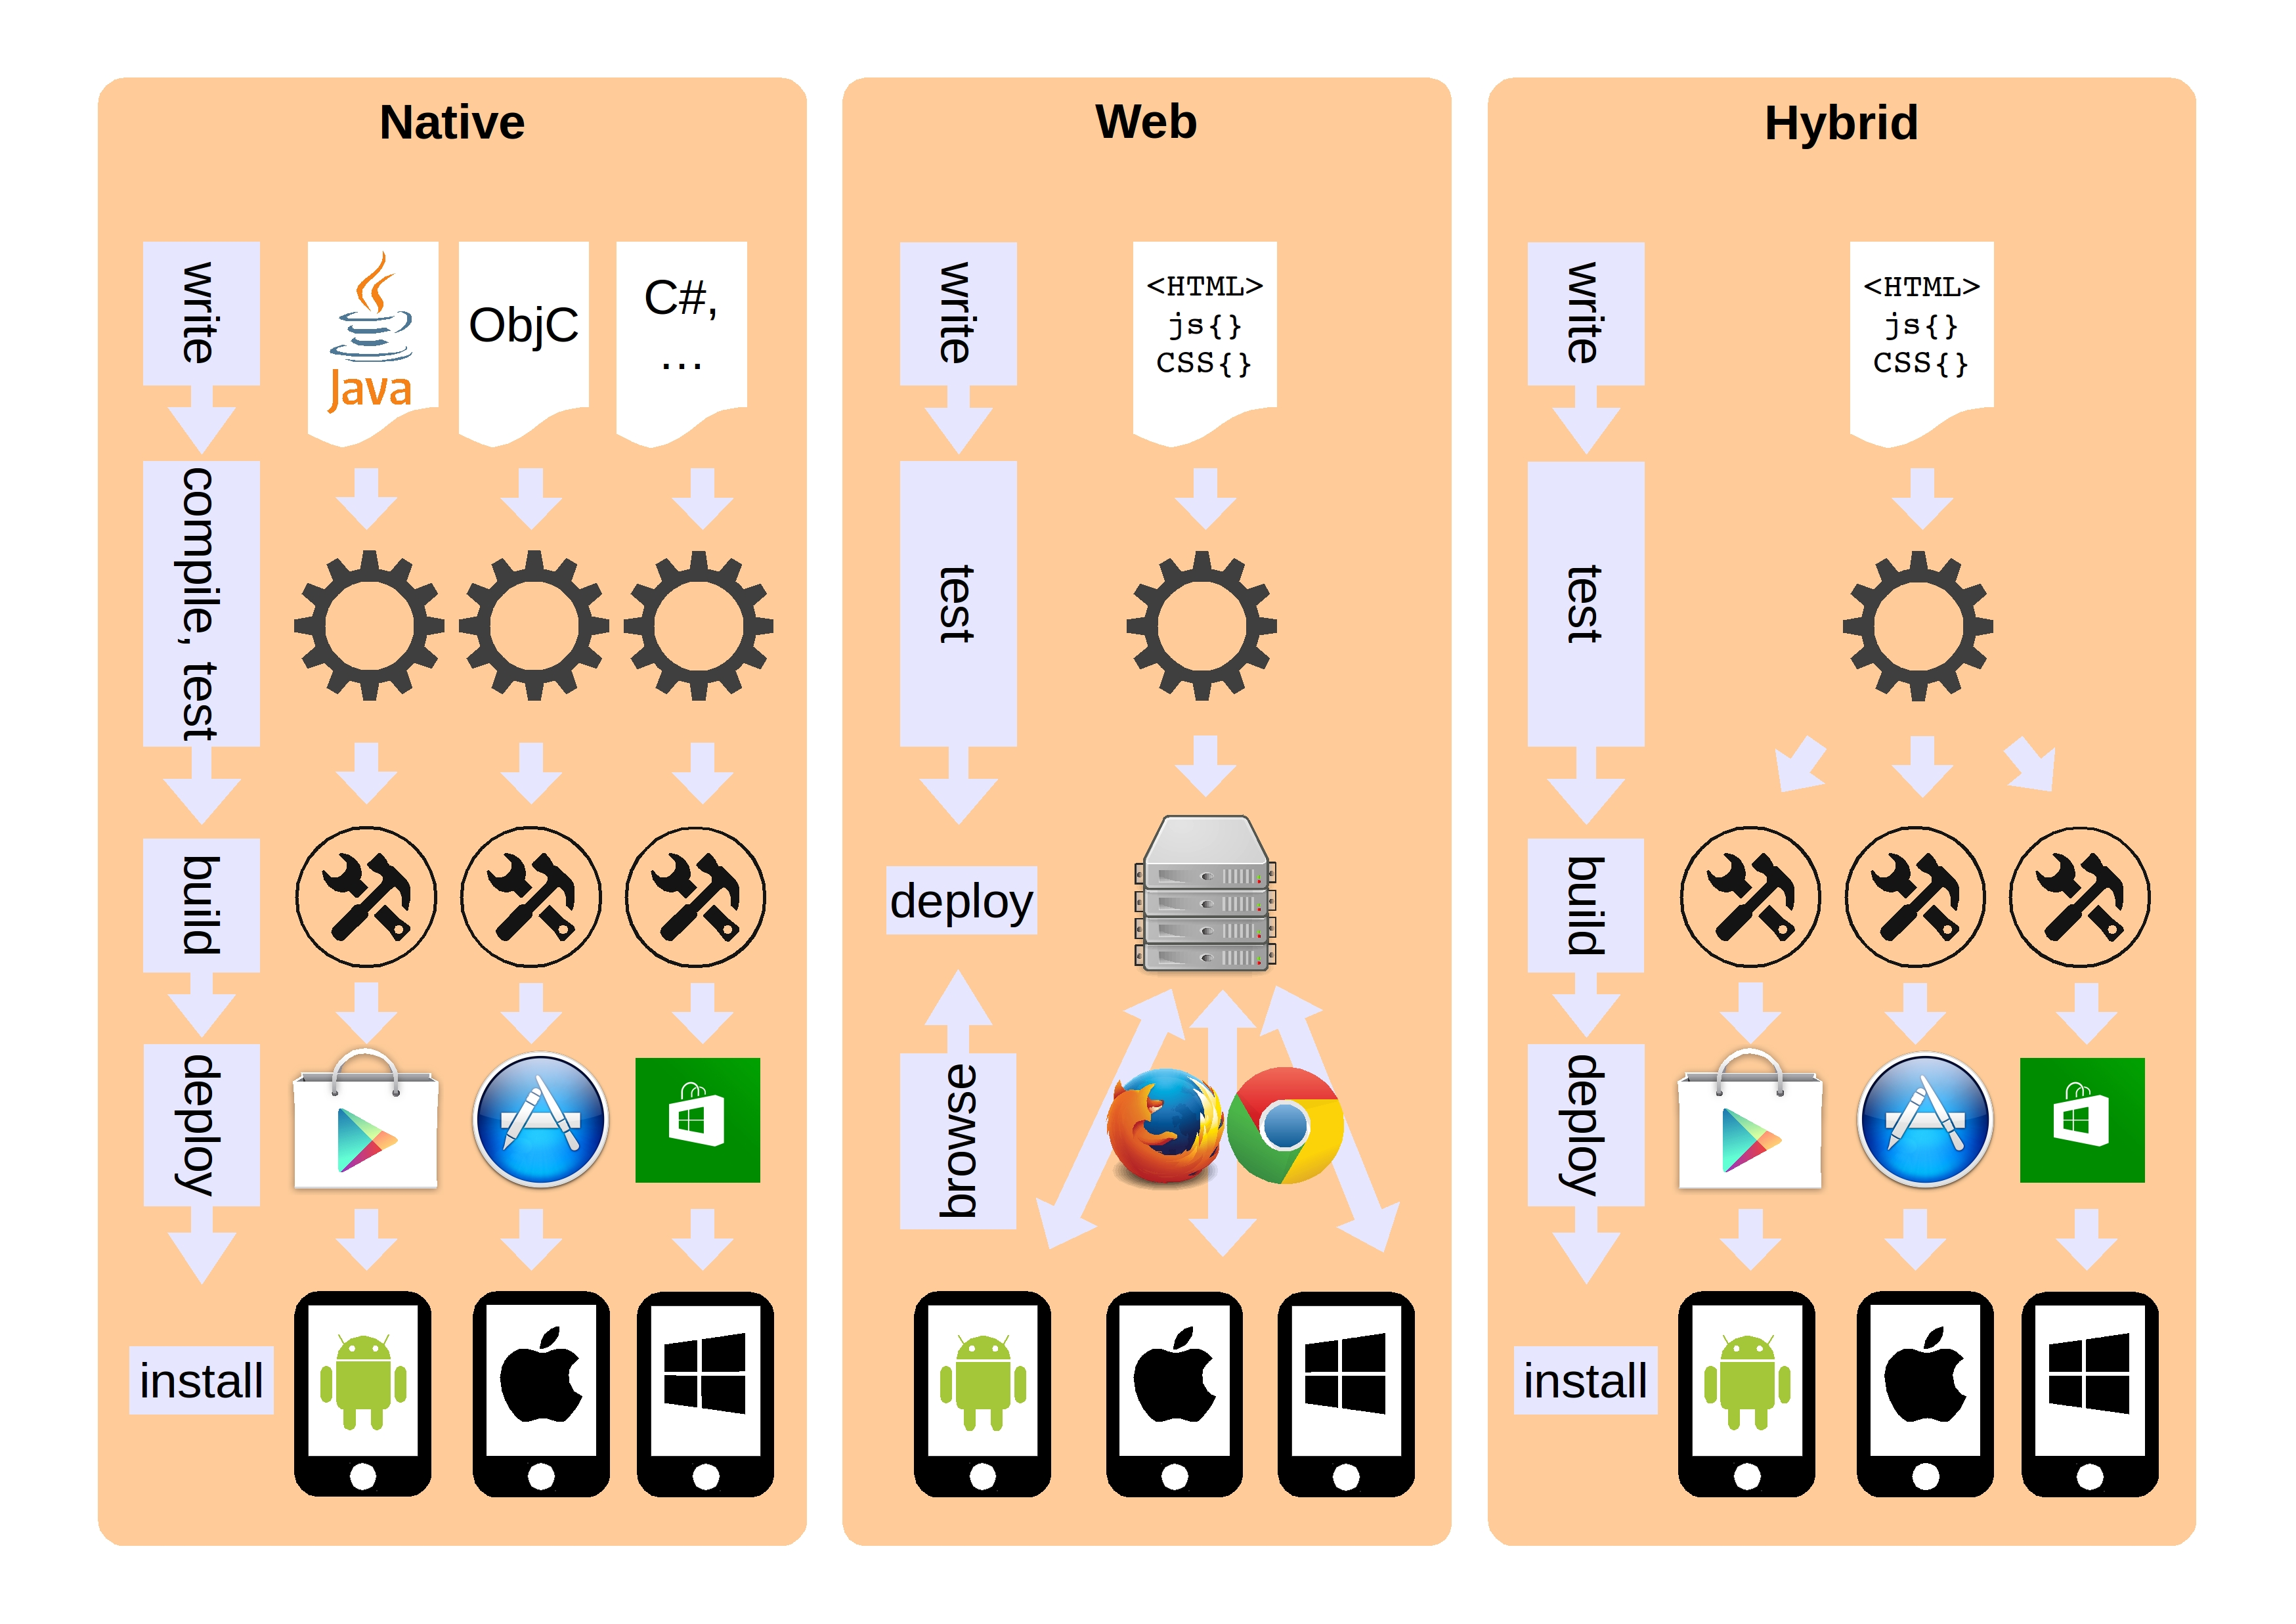
\includegraphics[width=1\textwidth,natwidth=1,natheight=1]{hybrid-apps-schaubild.jpg}
\caption[Schaubild Hybrid Apps]{Entwicklungsstufen der verschiedenen Arten von \glspl{app}. Während bei der nativen \gls{app} der gesamte Entwicklungszyklus einmal pro Plattform durchlaufen werden muss, verringert sich der Aufwand für die \gls{web-app} erheblich. Bei der \gls{hybrid-app} muss die Anwendung zwar einmal für jede Plattform gebaut und ausgeliefert werden um die Schnittstellen für die nativen Plattformen zu implementieren, aber der hauptsächliche Entwicklungsaufwand des Programmierens und Testens fällt aufgrund des generischen Charakters nur einmal an.}
\label{fig:hybrid-apps-schaubild}
\end{figure}

\section{Plattformunabhängige App-Entwicklung}

\subsection{Möglichkeiten des Erreichens von Plattformunabhängigkeit}

\subsection{Lösungen für die hybride App-Entwicklung}

\subsection{Entwicklung von hybriden Apps}\label{hybrid}

Wie in \ref{hybrid-app} beschrieben, bildet die hybride App-Entwicklung die Schnittmenge aus der nativen App-Entwicklung und der Web-Entwicklung mithilfe von Web-Technologien und zusätzlichen Frameworks und Bibliotheken. 
Hier soll mit \gls{phonegap} die konkrete Nutzung eines dieser Frameworks und weitere verwendete Technologien wie \gls{ko} oder \gls{jqm} erläutert werden.

Bereits für die Entwicklung von reinen Web-Anwendungen stellen neben den grundlegenden Web-Technologien \gls{html}, \gls{css} und \gls{js} Erweiterungen wie die JavaScript-Bibliothek \gls{jq} nützliche Hilfsmittel dar, die viele Funktionen gegenüber der Verwendung von \enquote{reinem} \gls{js} deutlich vereinfacht. %TODO BSP.!!
\todo{sollte das hier eher in \autoref{web-app}? Da es hier um die konkrete Erläuterung der Entwicklung geht, passt es aber vielleicht auch.}

\begin{lstlisting}[caption=Einbinden von JQuery in eine HTML-Seite, language=HTML, label=jq]
<html>
	<head>
		<title>Titel</title>
		<!-- hallo asdlfkj sdf -->
		<script src="lib/jquery-1.10.2.min.js"></script>
	</head>
	<body>
	[...]
	</body>
</html>
\end{lstlisting}

\subsubsection{JQueryMobile}



\subsubsection{KnockoutJS}



\subsubsection{Phonegap}

\gls{phonegap} ist ein Framework zur hybriden App-Entwicklung von \gls{adobe} und baut auf…

\subsubsection{PhoneGap Build}




\begin{comment}
Für letzteres bietet PhoneGap eine Javascript-Bibliothek, die auf das Cross-Platform-Framework \gls{cordova} von Apache aufbaut und den Zugriff auf native Features des jeweiligen Betriebssystems ermöglicht. \todo{wie genau, weiß ich noch nicht, noch rausfinden!}
Bei der konkreten Verwendung von nativen Features muss jedoch teilweise wieder auf die Unterstützung durch die jeweiligen Plattformen geachtet werden. \todo{oder zumindest muss deklariert werden, was verwendet werden soll. -> checken!}

Darüber hinaus übernimmt das Online-Portal \gls{pg-build} den Bauprozess der \gls{app}, also das Überführen in ein installierfähiges \gls{app}-Format. 
Während der Entwickler ohne diesen Build-Service die verschiedenen Toolkits aller Zielplattformen lokal verwalten müsste, um Cordova zu verwenden,\cite{phonegap-doc-cordova} reicht es hier aus, die Web-Anwendung (beispielsweise per öffentlichem Git-Repository) auf das Portal hoch zu laden, den Build-Prozess im Browser abzuwarten und die fertigen \glspl{app} auf das gewünschten Zielgerät herunterzuladen und zu installieren. 


\subsubsection{JQueryMobile}
Die Javascript-Bibliothek JQueryMobile baut auf JQuery auf und bietet ein Oberflächen-Toolkit für mobile Webseiten. Sie besteht zum Einen aus einer Javascript-Datei, die in die \gls{html}-Seite eingebunden wird und zum Anderen aus einem \gls{css}, das für das an mobile Touch-Geräte angepasste aussehen verantwortlich ist. 
So können einerseits UI-Elementen explizit Style-Klassen aus dem JQueryMobile-\gls{css} zugewiesen werden, andererseits sorgt das JQuery-Javascript ohnehin bei allen verwendeten \gls{html}-Elementen dafür, dass die Style-Klassen dynamisch vergeben werden und die UI-Komponenten somit ihr \gls{app}-typisches Aussehen erhalten.
Lediglich mit dem zusätzlichen Attribut \enquote{data-role} werden den UI-Elementen Eigenschaftentypen zugewiesen, über die die JQueryMobile-Bibliothek erkennt, wie dieses dargestellt werden soll.
\todo{Konkreter, Beispiel!}

Dieser Mechanismus erleichtert es dem Frontend-Entwickler erheblich, eine auf Touchscreens ausgerichtete Oberfläche zu entwerfen, da er im Grunde neben einigen zusätzlichen Attributen sämtliche herkömmlichen \gls{html}-Elemente verwenden kann. 

\subsubsection{KnockoutJS}
Auch bei \emph{Knockout} handelt es sich um eine Javascript-Bibliothek, die per \mbox{\texttt{<script>}-Tag} der \gls{html}-Seite hinzugefügt wird. Knockout übernimmt mit einem MVVM (Model-View-ViewModel) das \emph{Data-Binding}, also die Verknüpfung zwischen Daten-Feldern im Programm und UI-Elementen.
So lässt sich die UI (View) sehr klar von der Programmlogik (Model) trennen, was der Lesbarkeit, Erweiterbarkeit und Wartbarkeit der Software zugute kommt.

Statt also Javascript mit \gls{html}-String-Schnipseln zu vermischen, indem das \gls{dom} direkt manipuliert und UI-Elemente zur Laufzeit
\todo{gibt es bei javascript überhaupt eine laufzeit?} 
programmatisch erweitert werden, definiert der Entwickler in einem separaten Javascript ein View-Model und bindet mit dem \gls{html}-Attribut \enquote{data-bind} eine bestimmte View-Eigenschaft an ein Datenfeld aus dem View-Model.
\todo{Konkreter, Beispiel, Grafik.}
\end{comment}

